%% from aastex61.cls with a few tweaks to allow for the unique format required.
\documentclass{rnaastex}

\begin{document}

\title{Line broadening from spectral channel width and a response function}

%% Note that the corresponding author command and emails has to come
%% before everything else. Also place all the emails in the \email
%% command instead of using multiple \email calls.
\correspondingauthor{Eric Koch}
\email{ekoch@ualberta.ca}
\author[0000-0001-9605-780X]{Eric Koch}
\author[0000-0002-5204-2259]{Erik Rosolowsky}
\affiliation{University of Alberta, Department of Physics 4-183 CCIS, Edmonton AB T6G 2E1, Canada}


%% Note that RNAAS manuscripts DO NOT have abstracts.
%% See the online documentation for the full list of available subject
%% keywords and the rules for their use.
\keywords{}

%% Start the main body of the article. If no sections in the
%% research note leave the \section call blank to make the title.

\section{}

Observations of spectral-lines are affected by two systematic sources of line broadening: averaging over finite spectral channels and the spectral response function of the telescope. In this note, we compare different methods for inferring the line width of a single noiseless Gaussian to a forward-modelling approach that explicitly models for systematic line broadening.  We explore the bias in the line width from each method and show that approximate correction factors typically used in the literature do not correctly remove this bias.

Spectral-lines measured by an ideal spectrometer\footnote{Each channel is independent of each other.} are a weighted average of the line profile over the finite spectral channel. A Gaussian centered at $\mu$ with an amplitude of $A$ and width of $\sigma$ that is averaged over channels centered at $v$ with width $\Delta v$ has the form
\begin{equation}
    \label{eq:finite_gaussian}
    G(v) = \frac{A}{(\Delta v)^2} \left[ {\rm erf}\left( \frac{\mu - (v - \Delta v / 2)}{\sqrt{2}\sigma} \right) - {\rm erf}\left( \frac{\mu - (v + \Delta v / 2)}{\sqrt{2}\sigma} \right) \right].
\end{equation}
The average over the channel width will give an underestimate of the amplitude and an overestimate of $\sigma$ such that the integral over the line is conserved.  The bias in the measured amplitude and line width from the channel averaging becomes worse as $\Delta v \rightarrow \sigma$.

The top two panels in Figure \ref{fig:width_recovery_comparison} show that the Gaussian averaged over spectral channels (Eq. \ref{eq:finite_gaussian}) with $\Delta v = \sigma$ (i.e., Nyquist-sampled; orange dashed line) is broadened compared to the true Gaussian (solid translucent blue).  For comparison, we also show that a Gaussian sampled only at the channel centres (solid green) without accounting for the channel widths differs significantly from channel-averaged spectrum.  The panels show the same Gaussian with the peak centered on a spectral channel and at the edge of the spectral channel.  In the latter case, the amplitude and width are more biased than in the former case, demonstrating that the bias in the amplitude and line width depends on the channel width {\it and} where the peak is located relative to the channels.  The latter dependency cannot be known in observations a priori since it is a property of the observed source.

Line broadening from the finite channel width is often accounted for with a correction factor that is subtracted in quadrature from the measure line width.  An often-used correction factor is defined by \citet{cprops} as the effective width from setting the area of a Gaussian equal to the rectangular area over one channel:
\begin{equation}
    \label{eq:width_corr_fact}
    \sigma_{\rm response} \approx \frac{\Delta v_{\rm channel}}{\sqrt{2\pi}}.
\end{equation}
%Other authors have adopted larger correction factors XXX that GBT paper w/o the sqrt on the bottom XXX.

%  since we only consider a Gaussian shape here, we refer to the channel width ($\Delta v$) in terms of the standard deviation ($\sigma$) of the Gaussian

The second source of line broadening is the response function of the spectrometer.  An observed spectrum will be convolved by the response function that correlates nearby channels.  The channel correlation further broadens the spectrum.  It is also common to Hanning smooth data, which will also yield correlated spectral channels.  For some instruments, the response function is well-characterized \citep{rosolowsky2008}, particularly for instruments whose response functions significantly alters the observed line shape \citep[e.g.][]{martin2015}.  In the absence of an analytic expression for the response function, the typical channel-to-channel correlation can be used to approximate a Hanning-like response function. \citet{leroy2016} characterize the typical channel-to-channel correlation ($r$) and fit an empirical polynomial model relating the channel coupling $k$ from a three-element Hanning kernel ($[k, 1 - 2k, k]$) to $r$: $k\approx 0.0 + 0.47r - 0.23r^2 - 0.16r^3 + 0.43 r^4$. \citet{leroy2016} then extend Eq. \ref{eq:width_corr_fact} to account for correlated channels:
\begin{equation}
    \label{eq:leroy16_corrfact}
    \sigma_{\rm chan} \approx \frac{\Delta v}{\sqrt{2\pi}} \left( 1.0 + 1.18k + 10.4 k^2 \right).
\end{equation}
\citet{sun2018} give the channel correlations for a number of \co datasets of nearby galaxies. For the example here, we use $r=0.26$ ($k=0.11$) for the IRAM-30m CO(2-1) data of M33 \citep{druard2014}.  Using this approximation for a response function, we convolve the channel-averaged Gaussian (Eq. \ref{eq:finite_gaussian}) in Figure \ref{fig:width_recovery_comparison} to show how a realistic response function further broadens the Gaussian.

Both sources of line broadening are systematic and, when known, can be included in the model for the spectral-line.  Accounting for systematics in this way is known as {\it forward-modelling}, and is commonly-used for some spectral-line observations \citep{rosolowsky2008,martin2015}.  In our approach, we fit the ``observed'' Gaussian using Eq. \ref{eq:finite_gaussian} as the model and convolve this with the three-element Hanning kernel.  When the spectrum is noiseless, forward-modelling perfectly corrects for line broadening. 

While forward-modelling correctly accounts for line broadening, it requires directly fitting the spectrum, which can be computationally-expensive and requires a model to fit to.  Instead, many studies use approximate methods for calculating the line width, usually assuming a Gaussian shape.  We compare forward-modelling to four other methods: (1) Gaussian fitting without forward-modelling, (2) equivalent width: $\sigma_{\rm equiv} = A / \sqrt{2\pi} \Sigma$\footnote{$\Sigma$ is the integrated intensity of the line.} \citep{heyer2001,leroy2016,sun2018}, (3) second moment: $\sigma_{\rm Mom2}=\sqrt{\Sum_i T_i (v_i - v_0)^2 / \Sum_i T_i}$\footnote{Where $T_i$ is the value at $v_i$ and $v_0$ is the centroid.}, and (4) half-width-half-max (HWHM) from the locations where the spectrum is equal to half the peak \citep{stilp2013a,stilp2013b,koch2018}.

As a function of $\Delta v / \sigma$, we calculate the line width from each method, with and without subtracting a correction factor (Eqs. \ref{eq:width_corr_fact} \& \ref{eq:leroy16_corrfact}), for the channel-averaged Gaussian (Eq. \ref{eq:finite_gaussian}) with and without convolving by the spectral response function.  The bottom four panels in Figure \ref{fig:width_recovery_comparison} show the measured line widths.  The first column are line widths for a Gaussian centered on a channel.  We find that all approximate line width methods are similarly biased in this case.  Subtracting the correction factor from Eq. \ref{eq:width_corr_fact} overestimates the line broadening from the channel-averaging (second row), while the empirical correction factor from \citet{leroy2016} correctly removes the broadening when convolved with the response function to $<5\%$ (third row).

The second column shows line widths when the peak is centered at the edge of a channel. The different methods deviate in this case.  With no response function (second row), the Gaussian fit and second moment are similar to the when the peak is at the channel centre, and applying the correction factor overestimates the line broadening. The equivalent width and HWHM are biased to larger values than the latter two methods because they depend on the amplitude of the profile, which is underestimated more than than in the channel-centre case, and the correction factor {\ti underestimates} the line broadening.

With the response function (third row), the line widths are qualitatively the same as without the response function: the equivalent width and HWHM give a much larger line width than the Gaussian fit and second moment.  The empirical correction factor from \citet{leroy2016} works well for the latter two methods, but underestimates the line broadening for the former two methods.

There is little deviation from the true line width if $\Delta v / \sigma \gtsim 2$, and since the bias from line broadening will likely be smaller than the uncertainty in most data, there is no need to account for line broadening. 

When $\Delta v / \sigma \lesssim 2$, line broadening should be accounted for.  In all cases, the only method that correctly accounts for line width broadening is the forward-model fitting.  We recommend that this method be used whenever feasible.

If approximate methods must be used, our results indicate that: (1) fitting without forward-modelling or the second moment should be used, and (2) the correction factor must account for the response function \citep[Eq. \ref{eq:leroy16_corrfact}][]{leroy2016}.  These recommendations are only for {\it high signal-to-noise, single Gaussian spectra}.  Each of the methods will break down for certain cases. For example, the second moment is sensitive to noise and non-Gaussian line shapes \citep{koch2018}, while fitting requires a reasonable signal-to-noise. 

% The examples in Figure \ref{fig:width_recovery_comparison} do not include noise in the spectra.  We test the forward-modelling model in the presence of noise drawn to give a peak signal-to-noise of 5 in the spectrum.  The noisy spectrum is then convolved with the response function used above to correlate the noise.  Drawing 1000 iterations of noise, we find that the fitted parameters are not biased by line broadening.  However, the Levenberg-Marquadt algorithm used for the fitting assumes that the noise is uncorrelated.  We test whether breaking this assumption significantly underestimates the parameter uncertainties from the covariance matrix by calculating the fraction of iterations that the true parameter value lies within the $1\mbox{-}\sigma$ uncertainty range from the fit.  We find that true values are within the uncertainty range in $\sim70\%$ of the iterations, similar to the expected $68.2\%$ for the $1\mbox{-}\sigma$ range for a Gaussian distribution.  The lack of modelling for correlated errors should not significantly change the uncertainties.  The correlated noise may become more important if the spectral response function correlates channels beyond their nearest neighbours.  In that case, a Gaussian process can be used to model the correlated uncertainties XXX rasmussen and michaels XXX.


\begin{figure*}
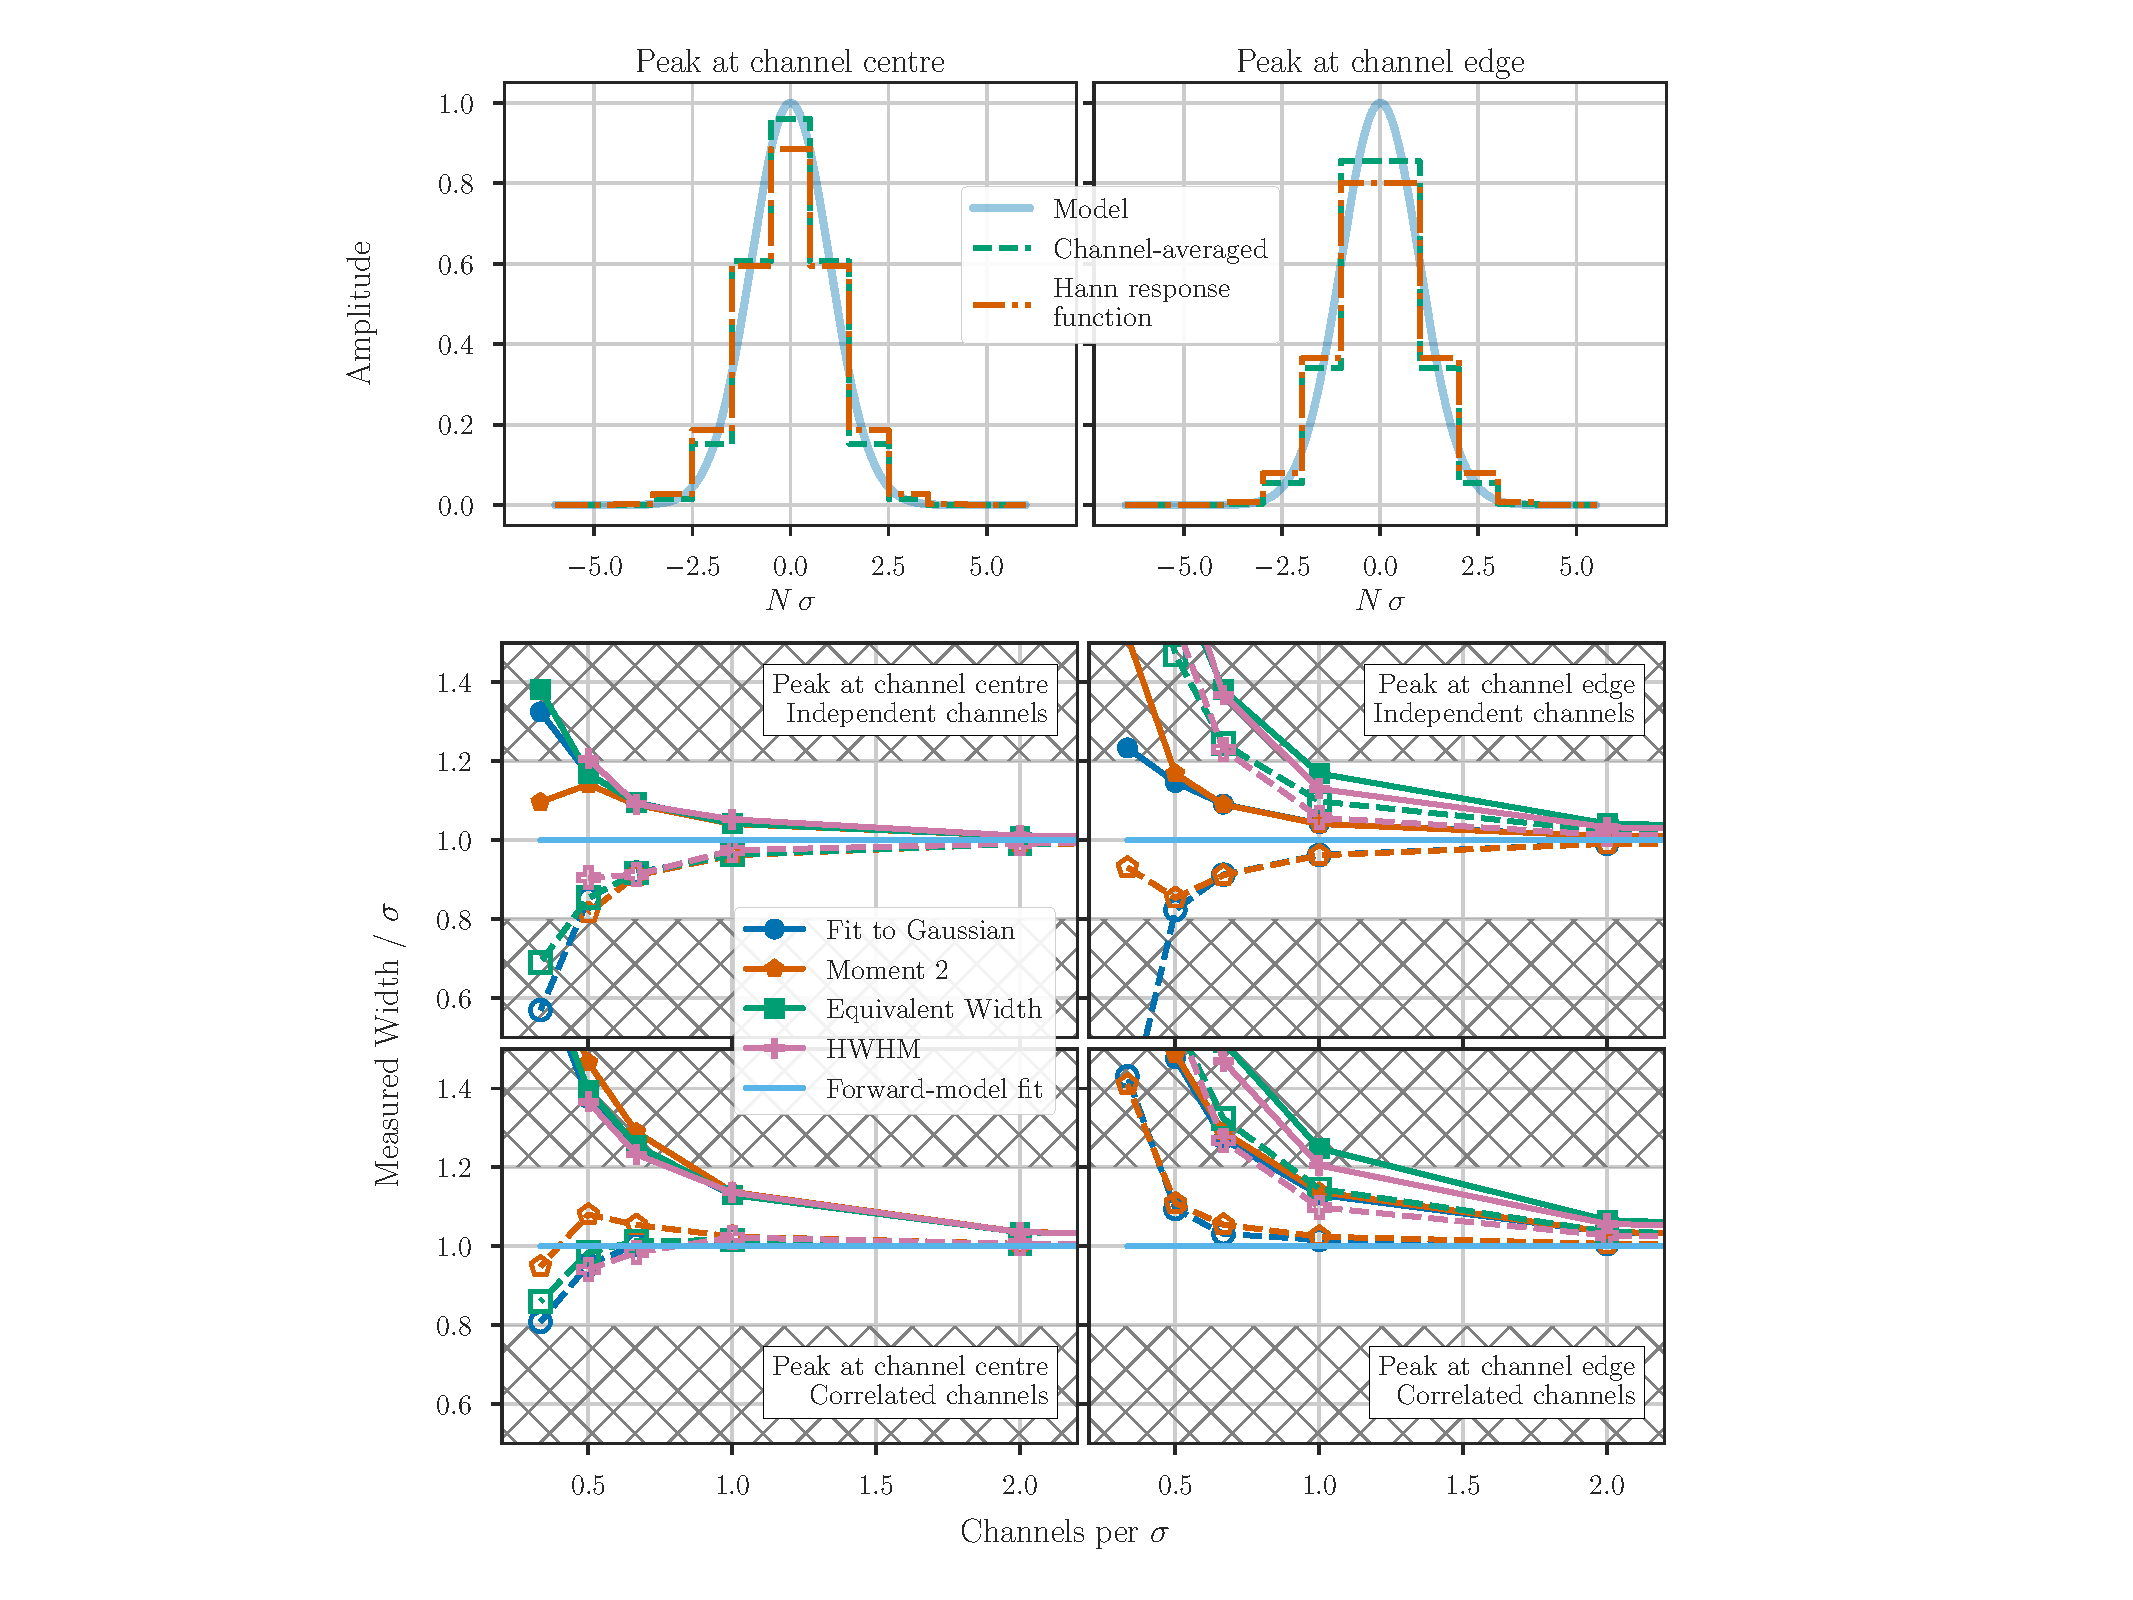
\includegraphics[width=\textwidth]{combined_figure}
\caption{\label{fig:width_recovery_comparison} XXX UPDATE FIGURE XXX Comparison of methods for recovering the width of a noiseless Gaussian model as a function of the number of channels per $\sigma$. The first row of panels show a Gaussian sampled with channels of $\Delta v=\sigma$ and how line broadening affects the shape.  The bottom two rows show the line widths measured with different methods, with a correction factor (dashed-unfilled) and without (solid). The middle row is from broadening from channel averaging and the bottom row is convolved with a Hanning response function with $k=0.11$. The first column shows results for a Gaussian at the channel centre and the second column is a Gaussian centred at the channel edge.  Where the peak is located with respect to the channels alters the line broadening.  We find that forward-modelling is the only method that correctly accounts for line broadening in all cases.}
\end{figure*}

The code to reproduce these results is available at: \url{https://github.com/Astroua/linewidth-corr-note}.

\acknowledgments

EWK is supported by a Postgraduate Scholarship from the Natural Sciences and Engineering Research Council of Canada (NSERC). EWR acknowledges the support of NSERC (RGPIN-2017-03987).

\software{XXX astropy, numpy, scipy, matplotlib, seaborn XXX}

\begin{thebibliography}{}

\bibitem[Druard et al.(2014)]{druard2014} Druard, C., Braine, J., Schuster, K.~F., et al.\ 2014, \aap, 567, A118.

\bibitem[Heyer et al.(2001)]{heyer2001} Heyer, M.~H., Carpenter, J.~M., \& Snell, R.~L.\ 2001, \apj, 551, 852.

\bibitem[Koch et al.(2018)]{koch2018} Koch, E.~W., Rosolowsky, E.~W., Lockman, F.~J., et al.\ 2018, \mnras, 479, 2505.

\bibitem[Leroy et al.(2016)]{leroy2016} Leroy, A.~K., Hughes, A., Schruba, A., et al.\ 2016, \apj, 831, 16.

\bibitem[Martin et al.(2015)]{martin2015} Martin, T., Drissen, L., \& Joncas, G.\ 2015, Astronomical Data Analysis Software an Systems XXIV (ADASS XXIV), 327.

\bibitem[Rosolowsky, \& Leroy(2006)]{cprops} Rosolowsky, E., \& Leroy, A.\ 2006, Publications of the Astronomical Society of the Pacific, 118, 590.

\bibitem[Rosolowsky et al.(2008)]{rosolowsky2008} Rosolowsky, E.~W., Pineda, J.~E., Foster, J.~B., et al.\ 2008, The Astrophysical Journal Supplement Series, 175, 509.

\bibitem[Stilp et al.(2013a)]{stilp2013a} Stilp, A.~M., Dalcanton, J.~J., Warren, S.~R., et al.\ 2013, \apj, 765, 136.

\bibitem[Stilp et al.(2013b)]{stilp2013b} Stilp, A.~M., Dalcanton, J.~J., Skillman, E., et al.\ 2013, \apj, 773, 88.

\bibitem[Sun et al.(2018)]{sun2018} Sun, J., Leroy, A.~K., Schruba, A., et al.\ 2018, \apj, 860, 172.


\end{thebibliography}

\end{document}
